\documentclass[tikz, border=10pt]{standalone}
\definecolor{mycolor}{HTML}{4965B0} % 正确定义颜色
\begin{document}
	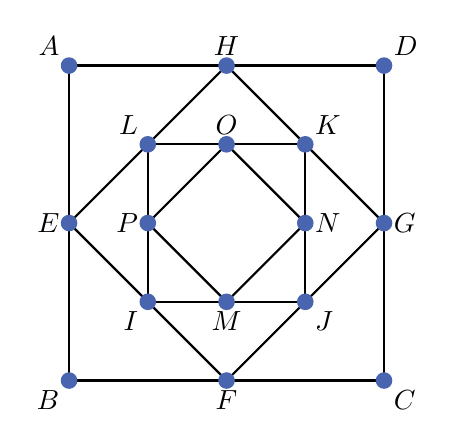
\begin{tikzpicture}[
		dot/.style={circle, fill=mycolor, minimum size=6pt, inner sep=0pt},
		line/.style={black, thick}
		]
		
		% 顶点坐标
		\coordinate (A) at (0, 4);
		\coordinate (B) at (0, 0);
		\coordinate (C) at (4, 0);
		\coordinate (D) at (4, 4);
		
		\coordinate (E) at (0, 2);
		\coordinate (F) at (2, 0);
		\coordinate (G) at (4, 2);
		\coordinate (H) at (2, 4);
		
		\coordinate (L) at (1, 3);
		\coordinate (K) at (3, 3);
		\coordinate (J) at (3, 1);
		\coordinate (I) at (1, 1);
		
		\coordinate (P) at (1, 2);
		\coordinate (M) at (2, 1);
		\coordinate (N) at (3, 2);
		\coordinate (O) at (2, 3);
		
		% 画线（黑色）
		\draw[line] (A) -- (B) -- (C) -- (D) -- cycle;
		\draw[line] (E) -- (F) -- (G) -- (H) -- cycle;
		\draw[line] (L) -- (I) -- (J) -- (K) -- cycle;
		\draw[line] (O) -- (P) -- (M) -- (N) -- cycle;
		
		% 画点（#4965b0填充，无描边）
		\node[dot] at (A) {};
		\node[dot] at (B) {};
		\node[dot] at (C) {};
		\node[dot] at (D) {};
		\node[dot] at (E) {};
		\node[dot] at (F) {};
		\node[dot] at (G) {};
		\node[dot] at (H) {};
		\node[dot] at (L) {};
		\node[dot] at (I) {};
		\node[dot] at (J) {};
		\node[dot] at (K) {};
		\node[dot] at (P) {};
		\node[dot] at (M) {};
		\node[dot] at (N) {};
		\node[dot] at (O) {};
		
		% 字母标注
		\node[above left] at (A) {$A$};
		\node[below left] at (B) {$B$};
		\node[below right] at (C) {$C$};
		\node[above right] at (D) {$D$};
		\node[left] at (E) {$E$};
		\node[below] at (F) {$F$};
		\node[right] at (G) {$G$};
		\node[above] at (H) {$H$};
		\node[above left] at (L) {$L$};
		\node[below left] at (I) {$I$};
		\node[below right] at (J) {$J$};
		\node[above right] at (K) {$K$};
		\node[left] at (P) {$P$};
		\node[below] at (M) {$M$};
		\node[right] at (N) {$N$};
		\node[above] at (O) {$O$};
		
	\end{tikzpicture}
\end{document}